%% Artículo final · Reto Ternium · Equipo Matacanes
%% Plantilla: elsarticle (Elsevier), formato de doble columna (5p) para Journal of Manufacturing Systems.
%% Compilar con pdfLaTeX + BibTeX (latexmk -pdf main.tex). Las cifras salen de generado/cifras.tex,
%% que regenera `python -m src.reproducir`; no se escriben números de resultados a mano en el texto.
\documentclass[5p,times,twocolumn]{elsarticle}

\usepackage[utf8]{inputenc}
\usepackage[T1]{fontenc}
\usepackage[spanish,es-tabla,es-nodecimaldot,es-noshorthands]{babel}
\usepackage{amsmath,amssymb}
\usepackage{graphicx}
\usepackage{booktabs}
\usepackage{array}
\usepackage{tabularx}
\usepackage{multirow}
\usepackage{dblfloatfix}   % permite floats de doble columna abajo de la página ([b])
\usepackage{xcolor}
\usepackage[colorlinks=true,linkcolor=black,citecolor=blue!50!black,urlcolor=blue!50!black]{hyperref}
\usepackage{microtype}

\DeclareUnicodeCharacter{2212}{\ensuremath{-}}  % signo menos tipográfico de las cifras generadas
\newcolumntype{L}[1]{>{\raggedright\arraybackslash}p{#1}}
\newcommand{\Y}{\ensuremath{Y}}
\newcommand{\pp}{\,pp}
\renewcommand{\arraystretch}{1.08}
% Floats de doble columna arriba o abajo de la página, nunca a media página (observación E1-02)
\renewcommand{\dbltopfraction}{0.85}
\renewcommand{\dblfloatpagefraction}{0.8}
\renewcommand{\topfraction}{0.85}
\renewcommand{\bottomfraction}{0.6}
\renewcommand{\textfraction}{0.1}
\renewcommand{\floatpagefraction}{0.8}
\setcounter{dbltopnumber}{3}
\setlength{\tabcolsep}{4pt}

% Generado por python -m src.reproducir a partir de outputs/tablas/cifras.json. No editar a mano.
\newcommand{\BendRealIQR}{239}
\newcommand{\BendRealPresetCero}{−57}
\newcommand{\CHKAnula}{0.025}
\newcommand{\CHRDConf}{51.6}
\newcommand{\CHRDRef}{34.0}
\newcommand{\CHRV}{1.47}
\newcommand{\CHRVa}{0.46}
\newcommand{\CHRYConf}{100.0}
\newcommand{\CHRYRef}{24.8}
\newcommand{\CHUnoEntre}{40}
\newcommand{\CoronaMedianaUm}{60}
\newcommand{\CoronaPcincoUm}{44}
\newcommand{\CoronaPnoventaycincoUm}{147}
\newcommand{\CoronaRelMediana}{2.04}
\newcommand{\CoronaRelMedianaDic}{3.42}
\newcommand{\CorrRealPreset}{0.53}
\newcommand{\CorrYPrimeraPieza}{0.98}
\newcommand{\DesfaseMedianoH}{125}
\newcommand{\ElongMediana}{1.51}
\newcommand{\EspesorMediano}{3.06}
\newcommand{\ExcGrupoMvMax}{27.0}
\newcommand{\ExcGrupoMvMin}{13.2}
\newcommand{\ExcProdMvMax}{12.5}
\newcommand{\ExcProdMvMin}{2.3}
\newcommand{\ExcesoAltDimension}{3.1}
\newcommand{\ExcesoAltProducto}{13.7}
\newcommand{\ExcesoAltPrograma}{26.3}
\newcommand{\ExcesoAltTipo}{0.2}
\newcommand{\ExcesoDimension}{4.0}
\newcommand{\ExcesoDimensionIC}{[3.1, 4.8]}
\newcommand{\ExcesoProdDim}{12.8}
\newcommand{\ExcesoProducto}{8.8}
\newcommand{\ExcesoProductoIC}{[7.0, 10.6]}
\newcommand{\ExcesoPrograma}{22.1}
\newcommand{\ExcesoProgramaIC}{[20.5, 23.6]}
\newcommand{\ExcesoTipo}{0.2}
\newcommand{\ExcesoTipoIC}{[0.0, 0.5]}
\newcommand{\ExpAbsY}{134.6}
\newcommand{\ExpAbsYCelda}{126.5}
\newcommand{\ExpAbsYGlobal}{127.3}
\newcommand{\ExpAbsYTipo}{127.3}
\newcommand{\ExpDeltaA}{8.0}
\newcommand{\ExpDeltaADE}{1.8}
\newcommand{\ExpDeltaB}{3.9}
\newcommand{\ExpDeltaDif}{0.8}
\newcommand{\ExpDeltaDifDE}{1.4}
\newcommand{\ExpDeltaGlobal}{7.2}
\newcommand{\ExpFamAProg}{2,093}
\newcommand{\ExpFamARollos}{6,895}
\newcommand{\ExpFamASemProg}{131}
\newcommand{\ExpFamASemRollo}{42.2}
\newcommand{\ExpFamBProg}{8,907}
\newcommand{\ExpFamBRollos}{29,344}
\newcommand{\ExpFamBSemProg}{557}
\newcommand{\ExpFamBSemRollo}{179.5}
\newcommand{\ExpFamDifProg}{199,634}
\newcommand{\ExpFamDifRollos}{657,694}
\newcommand{\ExpFamDifSemProg}{12,477}
\newcommand{\ExpFamDifSemRollo}{4,022.6}
\newcommand{\ExpFamProgSemana}{16}
\newcommand{\ExpFamRollosSemana}{164}
\newcommand{\ExpFamSigmaDentro}{119.2}
\newcommand{\ExpFamSigmaProg}{65.7}
\newcommand{\ExpFamilia}{DECAPADO · TER}
\newcommand{\ExpFamiliaRollos}{8,342}
\newcommand{\ExpMDEB}{8.0}
\newcommand{\ExpTodoAProg}{1,792}
\newcommand{\ExpTodoARollos}{6,203}
\newcommand{\ExpTodoASemProg}{94}
\newcommand{\ExpTodoASemRollo}{6.6}
\newcommand{\ExpTodoBProg}{7,625}
\newcommand{\ExpTodoBRollos}{26,399}
\newcommand{\ExpTodoBSemProg}{401}
\newcommand{\ExpTodoBSemRollo}{28.2}
\newcommand{\ExpTodoDifProg}{170,906}
\newcommand{\ExpTodoDifRollos}{591,702}
\newcommand{\ExpTodoDifSemProg}{8,995}
\newcommand{\ExpTodoDifSemRollo}{632.2}
\newcommand{\ExpTodoProgSemana}{19}
\newcommand{\ExpTodoRollosSemana}{936}
\newcommand{\ExpTodoSigmaDentro}{113.1}
\newcommand{\ExpTodoSigmaProg}{60.8}
\newcommand{\MedianaProgRodillo}{28}
\newcommand{\MedianaRollosPrograma}{62}
\newcommand{\NAsocCeldas}{4,451}
\newcommand{\NAsocProgramas}{828}
\newcommand{\NAsocRollos}{41,539}
\newcommand{\NCeldas}{6,137}
\newcommand{\NContrastes}{104}
\newcommand{\NDimensiones}{33}
\newcommand{\NExclCenso}{3,097}
\newcommand{\NExclSinCorona}{1,064}
\newcommand{\NExclSinY}{41}
\newcommand{\NInclusiones}{1,544}
\newcommand{\NOtras}{2,428}
\newcommand{\NPresetAlto}{1,733}
\newcommand{\NProdBH}{0}
\newcommand{\NProdGrandes}{35}
\newcommand{\NProdHet}{35}
\newcommand{\NProdHetRollos}{31,264}
\newcommand{\NProdICexcluyeCero}{1}
\newcommand{\NProdNeg}{27}
\newcommand{\NProductos}{331}
\newcommand{\NProgramas}{831}
\newcommand{\NRegistrosSKP}{58,786}
\newcommand{\NRegistrosSinLiga}{1,687}
\newcommand{\NRodillos}{35}
\newcommand{\NRollosAnalitica}{44,272}
\newcommand{\NRollosAsoc}{43,208}
\newcommand{\NRollosCenso}{44,313}
\newcommand{\NRollosDivididos}{8,526}
\newcommand{\NRollosMC}{149,734}
\newcommand{\NRollosRuta}{50,016}
\newcommand{\NRollosSKP}{47,410}
\newcommand{\NSinSoporte}{44}
\newcommand{\NSinSoporteRollos}{96}
\newcommand{\NVariantes}{15}
\newcommand{\NVariantesICCero}{1}
\newcommand{\NulaDimension}{2.6}
\newcommand{\NulaProducto}{0.9}
\newcommand{\NulaPrograma}{39.4}
\newcommand{\NulaTipo}{0.0}
\newcommand{\ObsDimension}{6.5}
\newcommand{\ObsProducto}{9.7}
\newcommand{\ObsPrograma}{61.4}
\newcommand{\ObsRollo}{22.1}
\newcommand{\ObsTipo}{0.2}
\newcommand{\PctCalienteEnSKP}{94.2}
\newcommand{\PctDecapadoEnSKP}{95.1}
\newcommand{\PctDefInspector}{5.6}
\newcommand{\PctDicEnSKP}{74.4}
\newcommand{\PctDivididos}{17.7}
\newcommand{\PctInclusiones}{3.6}
\newcommand{\PctModoElongacion}{94.9}
\newcommand{\PctOtrasEnSKP}{94.9}
\newcommand{\PctPresetCero}{11.1}
\newcommand{\PctPresetUnicoDos}{50}
\newcommand{\PctPresetUnicoTodos}{79}
\newcommand{\PctProgUnRodillo}{74.8}
\newcommand{\PctRealCeroPresetCero}{0.0}
\newcommand{\PctRetenido}{7.7}
\newcommand{\PctRetenidoSinCorona}{97.8}
\newcommand{\PctRetenidoSinDef}{3.8}
\newcommand{\PctRollosProdGrandes}{73.7}
\newcommand{\PctTensionEnrollado}{70}
\newcommand{\PctYMayorCincuenta}{59}
\newcommand{\PctYPorSD}{2.0}
\newcommand{\PendCorona}{−3.9}
\newcommand{\PendCoronaIC}{[−6.6, −1.2]}
\newcommand{\PendCoronaP}{0.005}
\newcommand{\PendCoronaSD}{−3.9}
\newcommand{\PendCoronaSDIC}{[−6.6, −1.2]}
\newcommand{\PendCoronaT}{−2.84}
\newcommand{\PendMvMax}{−2.2}
\newcommand{\PendMvMin}{−5.7}
\newcommand{\PendPreset}{0.1}
\newcommand{\PendPresetIC}{[−2.6, 2.8]}
\newcommand{\PendProdMax}{10.2}
\newcommand{\PendProdMin}{−30.0}
\newcommand{\PendRealPreset}{0.42}
\newcommand{\PendTemp}{−0.23}
\newcommand{\PendTempIC}{[−0.62, 0.15]}
\newcommand{\PredImpCorona}{0.98}
\newcommand{\PredImpCoronaRango}{2}
\newcommand{\PredImpPrimera}{Producto}
\newcommand{\PredImpPrimeraKN}{8.2}
\newcommand{\PredMAEBaseAleat}{130.5}
\newcommand{\PredMAEBaseGrupo}{135.1}
\newcommand{\PredMAEBaseTemp}{142.7}
\newcommand{\PredMAEDifGrupo}{−2.1}
\newcommand{\PredMAEDifGrupoDE}{0.8}
\newcommand{\PredMAEModAleat}{128.3}
\newcommand{\PredMAEModGrupo}{133.0}
\newcommand{\PredMAEModTemp}{143.6}
\newcommand{\PredMejoraClara}{no}
\newcommand{\PredMejoraGrupo}{5}
\newcommand{\PredNTempTest}{11,652}
\newcommand{\PredNTempTrain}{32,620}
\newcommand{\PredRBaseAleat}{0.09}
\newcommand{\PredRBaseGrupo}{0.03}
\newcommand{\PredRBaseTemp}{0.01}
\newcommand{\PredRDEModGrupo}{0.03}
\newcommand{\PredRModAleat}{0.12}
\newcommand{\PredRModGrupo}{0.07}
\newcommand{\PredRModTemp}{0.05}
\newcommand{\PresetPnoventaynueve}{700}
\newcommand{\PresetPuno}{−300}
\newcommand{\RParcialCorona}{0.02}
\newcommand{\RealPnoventaynueve}{446}
\newcommand{\RealPuno}{−348}
\newcommand{\SDCoronaDentro}{1.00}
\newcommand{\SecBendReal}{−3.78 [−6.03, −1.53]}
\newcommand{\SecDefInsp}{−0.22 [−0.45, 0.01]}
\newcommand{\SecElong}{0.00 [0.00, 0.00]}
\newcommand{\SecRetenido}{−0.14 [−0.50, 0.21]}
\newcommand{\VCuatroExcesoDia}{20.5}
\newcommand{\VCuatroExcesoDiaIC}{[19.2, 21.8]}
\newcommand{\VCuatroExcesoProg}{22.1}
\newcommand{\VCuatroExcesoProgIC}{[20.5, 23.6]}
\newcommand{\VCuatroExcesoRodillo}{13.2}
\newcommand{\VCuatroExcesoRodilloIC}{[11.8, 14.6]}
\newcommand{\VCuatroExcesoSemana}{13.4}
\newcommand{\VCuatroExcesoSemanaIC}{[12.0, 14.7]}
\newcommand{\VCuatroProductoDia}{8.8}
\newcommand{\VCuatroProductoProg}{8.8}
\newcommand{\VCuatroProductoRodillo}{8.8}
\newcommand{\VCuatroProductoSemana}{8.8}
\newcommand{\VDosCambio}{−3.7}
\newcommand{\VDosPdiez}{−0.57}
\newcommand{\VDosPnoventa}{0.38}
\newcommand{\VUnoCoef}{−0.3}
\newcommand{\VUnoCoefAj}{0.1}
\newcommand{\VUnoIC}{[−9.3, 8.7]}
\newcommand{\VUnoICAj}{[−8.9, 9.1]}
\newcommand{\VUnoP}{0.95}
\newcommand{\YDE}{191}
\newcommand{\YDEAsoc}{191}
\newcommand{\YMedia}{−99}
\newcommand{\YMediana}{−45}
\newcommand{\YMedianaSinCorona}{−48}
\newcommand{\YPcinco}{−517}
\newcommand{\YPnoventaycinco}{122}


\journal{Journal of Manufacturing Systems}

\begin{document}

\begin{frontmatter}

\title{La corrección de bending del Skinpass depende más del programa que del producto: evidencia de un año
de rollos ligados entre la laminación en caliente y la laminación de temple}

%% La Entrega I se firmó como "Grupo Matacanes". Si el profesor pide nombres, agregar un \author por integrante.
\author{Equipo Matacanes}
\affiliation{organization={Tecnológico de Monterrey, Escuela de Ingeniería y Ciencias},
             city={Monterrey}, state={Nuevo León}, country={México}}

\begin{abstract}
La laminación de temple (Skinpass) corrige la forma de la lámina laminada en caliente con un lazo de control de
bending que ajusta sobre una receta fija por tipo de material, y Ternium busca evidencia para decidir si conviene
diferenciar recetas por producto. Ligamos, rollo por rollo, un año de registros del Molino Caliente~4 y del Skinpass de
Pesquería (\NRollosAnalitica{} rollos en \NProgramas{} programas) y preguntamos qué tanto de la corrección que aplica el
lazo, el bending real menos el preset, se explica por el producto, la dimensión, el programa del Skinpass y la corona
relativa de salida del molino caliente. En una descomposición anidada contrastada con permutaciones, el programa explica
\ExcesoPrograma{} puntos porcentuales de la variación por encima del azar (IC~95\,\% \ExcesoProgramaIC), contra
\ExcesoProducto{} \ExcesoProductoIC{} del producto, y agrupar por día da casi lo mismo. Dentro de producto, dimensión y
mes, cada punto porcentual de corona relativa se asocia con una corrección \PendCorona~kN más negativa (IC~95\,\%
\PendCoronaIC), con el signo físico esperado, un control negativo nulo y la misma dirección en \NVariantes{}
alternativas de depuración y agrupación; pero el efecto es pequeño y un confusor no medido con 1/\CHUnoEntre{} de la fuerza del
producto lo anularía. Con validación agrupada por programa y temporal, un modelo de gradient boosting no anticipa la
corrección claramente mejor que la media por producto y dimensión. Recentrar el preset con la corrección histórica
bajaría su magnitud unos \ExpDeltaA~kN, y diferenciarlo por producto agregaría solo \ExpDeltaDif~kN. Antes de
diferenciar recetas, proponemos una operación evolutiva rollo a rollo dentro de cada programa (\ExpTodoARollos{}
rollos, unas \ExpTodoASemRollo{} semanas de producción) y el registro de la planeza de salida, que hoy no se mide.
\end{abstract}

\begin{keyword}
laminación de temple \sep Skinpass \sep bending \sep corona \sep datos observacionales \sep descomposición de la
varianza \sep operación evolutiva
\end{keyword}


\end{frontmatter}

\section{Introducción}
\label{sec:intro}

\paragraph{Contexto industrial}
La lámina de acero plano que llega a un cliente automotriz, de electrodomésticos o de construcción pasa por una
cadena de procesos en la que cada etapa hereda la geometría y el estado mecánico que deja la anterior. En la planta
de Pesquería de Ternium, el primer eslabón de esa cadena para el producto laminado es el \emph{Molino Caliente~4}
(MC4): un planchón recalentado se desbasta y pasa por un tren acabador de siete castillos hasta convertirse en una
banda de pocos milímetros (espesor mediano de \EspesorMediano{}~mm en los rollos de este estudio), que se enfría en la
mesa de salida y se enrolla. La banda no sale perfectamente plana ni de espesor uniforme a lo ancho: suele ser más
gruesa al centro que en las orillas (\emph{corona}) y puede ser más gruesa de un lado que del otro (\emph{cuña}). El
espesor y la corona son los indicadores de desempeño más críticos de la laminación en caliente~\cite{peng2014}.

Varios días después (\DesfaseMedianoH{}~h de mediana en nuestros datos), una parte de esos rollos pasa por el
\emph{Skinpass} de Pesquería, una laminación de temple: una pasada en frío con una reducción muy pequeña, del orden
de 1\,\%~\cite{kijima2008}, y con tensión aplicada. Su propósito es suprimir el punto de cedencia discontinuo que
produce las bandas de Lüders en el conformado posterior, dar el acabado superficial y corregir la forma de la
lámina~\cite{lenard2014}. Para lo último, la palanca principal es el \emph{bending}: la fuerza que dobla los rodillos de
trabajo y cambia el perfil del claro entre ellos y, con ello, cuánto se alarga cada fibra de la lámina a lo ancho. Si
las fibras se alargan de manera desigual quedan esfuerzos residuales que se manifiestan como ondas de orilla o
pandeo central. Por eso la laminación de temple puede corregir una planeza no uniforme que trae el material, pero
también puede revelarla o crearla, y la planeza no uniforme de entrada es una de sus dificultades
reconocidas~\cite{lenard2014}. En la línea estudiada, cada rollo recibe un valor de bending de receta (\emph{preset})
y un lazo de control lo ajusta durante el proceso.

\paragraph{La decisión de Ternium}
Según el Socio Formador, hoy el Skinpass trabaja con una configuración por tipo de material (caliente, decapado o frío) aplicada a todos los
productos de esa familia. La receta única simplifica la operación, pero supone que productos distintos responden de
forma parecida a la misma configuración. Ternium preguntó qué combinación de parámetros del Skinpass se asocia con la
mejor calidad para cada producto y condición de entrada, para decidir si conviene diferenciar recetas por producto.
La decisión es real y tiene un costo: cada receta adicional se diseña, se valida y se mantiene. Contestarla con
historia de planta exige más que mostrar que los productos llegan distinto: exige saber qué pasaría con un producto si
se le cambiara la receta, una predicción contrafactual y no una descripción~\cite{hernan2019}, y mostrar que productos
distintos responden distinto a la misma receta (una interacción), no solo que parten de niveles distintos.

\paragraph{El giro como hallazgo}
Nuestra primera entrega encontró que esa pregunta, tal como está planteada, no puede contestarse con los registros
que existen, y documentar por qué fue el primer resultado del proyecto. Los 24 archivos iniciales describían el MC4,
no el Skinpass (sus cinco columnas del Skinpass venían vacías). Al obtener los resúmenes por rollo del Skinpass de
2025 y ligarlos con el MC4 aparecieron los otros dos obstáculos: el Skinpass no registra planeza de salida, de modo
que no hay un resultado de calidad de forma contra el cual comparar configuraciones, y el bending real no es una
palanca libre, sino la respuesta de un lazo cerrado a la forma de la lámina. Muchos proyectos industriales de
analítica fallan precisamente por no reconocer esa brecha entre la pregunta y los datos y por optimizar un modelo
predictivo como si sus coeficientes fueran efectos~\cite{box1966,shmueli2010}.

Lo que sí registran los datos es cuánto tuvo que corregir el lazo sobre la receta: la diferencia entre el bending
real y el preset, que llamamos $\Y$. Si la receta anticipara lo que el rollo necesita, $\Y$ sería cero. La pregunta
respondible que sigue importando para la decisión es, entonces:
\emph{en los rollos que el MC4 envió al Skinpass de Pesquería en 2025, ¿qué tanto depende la corrección de bending
de lo que se sabe antes de procesarlos ---su producto, su dimensión, el programa del Skinpass y la corona relativa
con que salen del MC4--- y cuál de esas fuentes pesa más?} Aquí, el \emph{programa} es la tanda de rollos que el
Skinpass procesa de corrido (con mediana de \MedianaRollosPrograma{} rollos), y la \emph{corona relativa} es la corona
dividida entre el espesor, en puntos porcentuales (pp). Si la corrección depende sobre todo del producto, una receta
por producto podría absorberla; si depende de otra cosa, diferenciar por producto no la absorbería.

\paragraph{Contribuciones}
Cada una se verifica en la sección~\ref{sec:resultados}:
\begin{enumerate}
\item Una unión verificada, rollo por rollo, entre el MC4 y el Skinpass de un año de producción
      (\NRollosAnalitica{} rollos en \NProgramas{} programas), con la población documentada paso a paso y las
      exclusiones comparadas contra los incluidos.
\item Una descomposición de la corrección de bending contra el azar: el programa del Skinpass explica
      \ExcesoPrograma{}\,\% de su variación por encima de lo que daría el azar, frente a \ExcesoProducto{}\,\% del producto
      y \ExcesoDimension{}\,\% de la dimensión; agrupar por día da casi lo mismo que por programa.
\item Una asociación ajustada entre la corona relativa del MC4 y la corrección, con el signo físico esperado pero
      pequeña (\PendCorona{}~kN por punto porcentual) y frágil ante confusión no medida, sometida a un control negativo,
      a \NVariantes{} alternativas de depuración y agrupación y a un análisis de sensibilidad.
\item Una evaluación predictiva honesta: con validación por programa y temporal, la información previa al Skinpass no
      anticipa la corrección claramente mejor que una receta por producto y dimensión.
\item Una propuesta de experimento evolutivo por programa, con su volumen estimado, y la lista de datos del Skinpass
      que harían respondible la pregunta original.
\end{enumerate}
Mostramos que la corrección que el lazo de bending aplica sobre la receta depende más del programa del Skinpass, y del
periodo en que se procesa el rollo, que del producto, y que la condición de salida del MC4 apenas la anticipa.

\section{Revisión de literatura}
\label{sec:literatura}

\subsection{Perfil y planeza: lo que la laminación en caliente le entrega al Skinpass}
En la laminación en caliente, el espesor y la corona son los indicadores de calidad que más pesan en la
rentabilidad~\cite{peng2014}, y la literatura de procesos los trata como resultados que el molino debe controlar. La
planeza, en cambio, depende de la distribución de alargamientos a lo ancho: una banda cuya corona no guarda
proporción con la del claro entre rodillos se alarga de manera desigual y acumula esfuerzos residuales que más tarde
aparecen como ondas o pandeo, y la planeza no uniforme con que llega la banda es una dificultad reconocida de la
laminación de temple~\cite{lenard2014}. Esa es la conexión física que motiva este trabajo: la corona con que
sale el rollo del MC4 debería importar para el Skinpass, porque fija cuánta elongación diferencial tendría que
compensar la pasada de temple. Pero en una planta la corona no es una variable libre. Depende del pedido (espesor y
ancho objetivo, grado), del estado de los rodillos del molino y del periodo de producción, de modo que cualquier
comparación entre rollos con distinta corona compara también pedidos y momentos distintos. La literatura de
laminación explica el mecanismo; no dice cuánto de ese mecanismo sobrevive a la mezcla de pedidos de un año real.

\subsection{La laminación de temple}
Los modelos de la laminación de temple coinciden en que es un proceso difícil de describir con la teoría clásica de
laminación plana. Con reducciones tan pequeñas, las regiones elástica y plástica de la banda son comparables, el
aplanamiento de los rodillos de trabajo domina las fuerzas y la reducción es del mismo orden que la rugosidad
superficial; por eso los modelos tradicionales predicen mal las fuerzas de separación y deben incorporar la
deformación del rodillo y fricción alta~\cite{lenard2014}. Kijima y Bay~\cite{kijima2008} ilustran la escala del
problema: con simulaciones de elementos finitos de una indentación plana, estudian cómo se transfiere la rugosidad del
rodillo a la lámina y cuánto se alarga ésta bajo carga normal pura, en un régimen de fricción seca y deformación muy
inhomogénea. Otros modelos tratan el molino de temple como un sistema de control de múltiples entradas y salidas, con
las tensiones, la fuerza y la velocidad como variables acopladas~\cite{lenard2014}. En conjunto, esta literatura
explica qué pasa dentro de una pasada y cómo controlarla; su unidad es el contacto rodillo--lámina o la línea en
estado estable, no la población de rollos de una planta. No responde, ni pretende hacerlo, cuánto difiere entre
productos la corrección que necesita el Skinpass cuando opera con una sola receta.

\subsection{Datos de proceso y datos de ocasión}
Los registros de planta son datos que nadie diseñó para contestar preguntas causales. Box~\cite{box1966} lo advirtió
para la regresión con datos no planeados: el término de error contiene variables latentes que cambian junto con las
variables observadas, y el coeficiente estimado mezcla el efecto buscado con el de esas variables; para saber qué
pasa cuando se interviene un sistema hay que intervenirlo. La literatura de monitoreo basado en datos en laminación
en caliente aprovecha bien esos registros para vigilar indicadores~\cite{peng2014}, porque su objetivo es detectar
desviaciones, no estimar qué pasaría con otra configuración. Hernán, Hsu y Healy~\cite{hernan2019} ordenan esta
distinción en tres tareas: describir, predecir y predecir contrafactuales; solo la tercera contesta "¿qué pasaría si
cambiamos la receta?", y exige supuestos que los datos de ocasión rara vez cumplen. Nuestra pregunta se ubica a
propósito en las dos primeras.

\subsection{Inferencia con datos observacionales}
Cuando se quiere ir más allá de la descripción, la literatura de inferencia observacional pide tres cosas. Primero,
comparar unidades comparables: ajustar por las variables que determinan la exposición y verificar que haya
traslape entre grupos antes de estimar~\cite{rosenbaum1983}. Segundo, que la incertidumbre respete la estructura de
los datos: con observaciones agrupadas, los errores estándar ingenuos subestiman la incertidumbre y deben agruparse
al nivel en que se asigna la variación~\cite{cameron2015}, y las fuentes jerárquicas de variación se describen mejor
con modelos multinivel que con un solo término de error~\cite{gelman2007}. Tercero, validar sin verdad de terreno:
controles negativos que no deberían responder a la exposición~\cite{lipsitch2010}, análisis de multiverso que muestren
juntas las alternativas razonables de depuración~\cite{steegen2016} y análisis de sensibilidad que digan qué tan
fuerte tendría que ser un confusor no medido para anular la conclusión, idealmente contra un confusor observado de
referencia~\cite{cinelli2020,vanderweele2017}. Cuando se examinan muchos grupos, el control de la tasa de
descubrimientos falsos~\cite{benjamini1995} y la agregación parcial~\cite{gelman2012} limitan los hallazgos espurios,
y elegir el grupo con el mejor resultado sobrestima su efecto: la maldición del optimizador~\cite{smith2006}. Estas
herramientas se desarrollaron sobre todo en epidemiología y economía; su aplicación a la cadena de laminación es
escasa, y es lo que este trabajo intenta.

\subsection{Aprendizaje automático en manufactura}
El aprendizaje automático promete extraer patrones de procesos complejos y ya tiene aplicaciones exitosas en
manufactura, pero su adopción enfrenta dos retos comunes: conseguir datos relevantes, cuya disponibilidad, calidad y
composición condicionan el desempeño, e interpretar los resultados~\cite{wuest2016}. Dos riesgos son específicos de nuestro caso. El primero es la fuga de
información: variables posteriores al resultado o etiquetas generadas por reglas sobre las mismas mediciones inflan
el desempeño y producen modelos inútiles en operación~\cite{kaufman2012,kapoor2023}. El segundo es la validación: si
rollos del mismo programa quedan a la vez en entrenamiento y prueba, el modelo aprende el programa y no el rollo, y
el desempeño reportado es optimista; las particiones deben respetar el tiempo y los grupos~\cite{roberts2017}. Aun
evitando ambos riesgos, un buen modelo predictivo no es un modelo explicativo: la importancia de una variable dice
qué usa el modelo para predecir, no qué pasaría al intervenirla~\cite{shmueli2010}.

\subsection{Síntesis y vacío}
\label{sec:vacio}
Las cinco líneas coinciden en algo que rara vez se dice junto. La física de la laminación explica por qué la forma
de entrada debería importar al Skinpass~\cite{lenard2014}, pero la literatura que revisamos la estudia dentro de una
pasada y no con la población de rollos de una planta~\cite{kijima2008}. Los datos de planta permiten describir esa
población, pero no contestar por sí solos qué receta sería mejor~\cite{box1966,hernan2019}.

Eso responde por qué la optimización de parámetros con aprendizaje automático no resuelve por sí sola el problema de
Ternium. Un modelo que predice la calidad a partir del producto y de la configuración, y que después se optimiza,
aprende qué configuraciones tuvieron los rollos que salieron bien bajo la regla histórica de asignación, no qué pasaría
si se cambiara la receta~\cite{hernan2019,shmueli2010}. Con una receta por tipo de material, casi no hay variación de
configuración dentro de cada producto, de modo que el modelo extrapola fuera del soporte observado. El bending real
lo fija un lazo que reacciona a la forma del rollo, lo que lo convierte en mediador y no en palanca. Y sin planeza de
salida no hay un resultado de forma que optimizar.

El vacío concreto que atendemos es previo a cualquier optimización: no encontramos, en la literatura revisada, una
medición de cuánto de la corrección que aplica el lazo de bending del Skinpass se explica por el producto y cuánto por
el programa o el periodo, a partir de datos ligados entre el molino caliente y el de temple. Esa cantidad acota lo que
una receta por producto podría absorber, y es la que este artículo estima.

\section{Datos y metodología}
\label{sec:metodologia}

Todas las decisiones de esta sección se fijaron en un plan de análisis escrito antes de la estimación principal; los
cambios posteriores, con su fecha y su motivo, están en la bitácora del plan (Anexo~\ref{sec:anexo-plan}).

\subsection{Proceso, fuentes y unión}
\label{sec:datos}

\begin{figure*}[t]
\centering
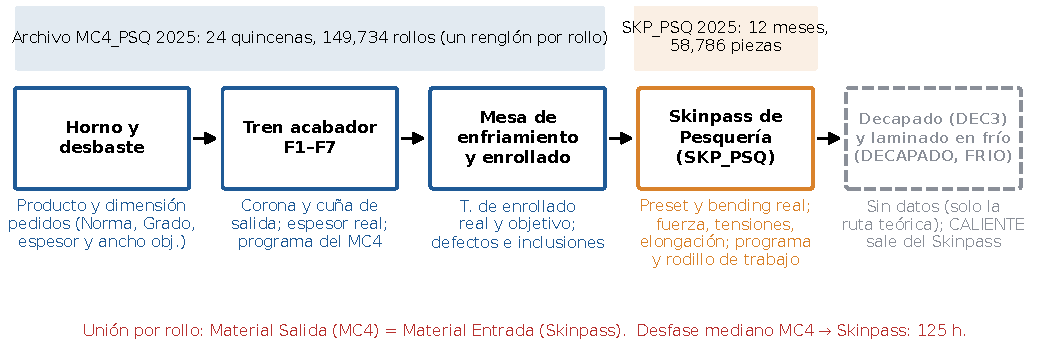
\includegraphics[width=\textwidth]{figuras/mapa_proceso.pdf}
\caption{\textbf{Cada rollo del MC4 llega al Skinpass varios días después, y sus dos registros se ligan rollo por
rollo.} Pregunta que responde: ¿en qué etapa nace cada dato que usamos? Se lee de izquierda a derecha, en el orden
en que viaja el acero. Bajo cada etapa están los datos que usamos (azul: archivo del MC4; naranja: archivo del
Skinpass). El decapado y la laminación en frío van después del Skinpass y no tienen datos.}
\label{fig:mapa}
\end{figure*}

Usamos dos fuentes de Ternium para todo 2025 (Fig.~\ref{fig:mapa}). La primera son 24 archivos quincenales del MC4
con un renglón por rollo (\NRollosMC{} rollos, 280 columnas): especificación del pedido, temperaturas, perfil de salida
y defectos. La segunda son 12 archivos mensuales del Skinpass de Pesquería con un renglón por pieza procesada
(\NRegistrosSKP{} registros, 208 columnas): programa, rodillo de trabajo, modo del molino, preset y valor real
promedio de bending, fuerza y tensiones, elongación, dictamen y defectos. La llave de unión es el identificador de
salida del MC4, que el Skinpass registra como material de entrada. Un rollo puede salir del Skinpass en varias piezas
(\NRollosDivididos{} rollos, \PctDivididos\,\%); las variables numéricas se agregan por rollo como promedio ponderado
por el peso de cada pieza, las banderas como ``alguna pieza'' y el programa, la fecha y el rodillo son los de la
primera pieza (las piezas comparten programa en todos los casos salvo uno). No ligan \NRegistrosSinLiga{} registros
del Skinpass, en su mayoría reprocesos de piezas ya pasadas y rollos laminados a fines de 2024; se cuentan por motivo
en el repositorio y se excluyen.

\subsection{Población y unidad de análisis}
\label{sec:poblacion}

\begin{table}[t]
\centering
\caption{Población de estudio paso a paso. Cada paso conserva los rollos que cumplen su criterio y los anteriores.
Progr.~SKP: programas del Skinpass distintos.}
\label{tab:poblacion}
\footnotesize
\begin{tabular}{cL{3.15cm}rrr}
\toprule
Paso & Criterio & Rollos & Excluidos & Progr. SKP \\
\midrule
0 & Rollos del MC4 en 2025 & 149,734 & -- & -- \\
1 & Ruta teórica con SKP\_PSQ (cualquier forma final) & 50,016 & 99,718 & -- \\
2 & Con registro en el Skinpass 2025 & 47,410 & 2,606 & 858 \\
3 & Laminados antes del 1-dic-2025 (censura) & 44,313 & 3,097 & 831 \\
4 & Con bending real y preset (Y definido) & 44,272 & 41 & 831 \\
5 & Además con corona relativa válida & 43,208 & 1,064 & 831 \\
\bottomrule
\end{tabular}

\end{table}

La Tabla~\ref{tab:poblacion} muestra cuántos rollos quedan en cada paso. Incluimos los rollos de \emph{cualquier}
forma final con el Skinpass de Pesquería en su ruta teórica, incluidos los \NOtras{} de formas finales que no terminan
en ``SKP'' y que la Entrega~I había excluido sin justificación: pasan por el Skinpass en la misma proporción
(\PctOtrasEnSKP\,\%) que los de forma final caliente (\PctCalienteEnSKP\,\%) o decapada (\PctDecapadoEnSKP\,\%).
Cortamos en los rollos laminados antes del 1 de diciembre porque solo \PctDicEnSKP\,\% de los de diciembre aparece en
el Skinpass de 2025; el resto se procesó en enero de 2026. Los excluidos por ese corte no son como los demás (corona
relativa mediana de \CoronaRelMedianaDic\,\% contra \CoronaRelMediana\,\%), así que el corte entra en el análisis de
robustez. Los \NExclSinCorona{} rollos sin corona válida quedan fuera solo de la asociación; casi todos fueron
retenidos en el MC4 (\PctRetenidoSinCorona\,\%, porque la regla de ``mal perfil'' se activa cuando falta la corona),
pero su corrección mediana es parecida a la del resto (\YMedianaSinCorona{} contra \YMediana~kN): la exclusión no depende
del resultado.

La unidad de análisis es el rollo del MC4, y siempre reportamos rollos y programas del Skinpass (\NProgramas{}
programas, con mediana de \MedianaRollosPrograma{} rollos). El \emph{producto} es la combinación de norma y grado
(\NProductos{} productos); la \emph{dimensión}, el rango de espesor objetivo por el rango de ancho objetivo del pedido
(valores especificados, no medidos); el \emph{tipo de material}, caliente, decapado o frío. Llamamos \emph{celda} a
cada combinación de producto, dimensión y mes (\NCeldas{} celdas).

\subsection{Resultado y variables que no pueden explicarlo}
\label{sec:resultado}
El resultado principal es la corrección de bending,
\begin{equation}
\Y_i = B^{\mathrm{real}}_i - B^{\mathrm{preset}}_i \quad [\mathrm{kN}],
\label{eq:y}
\end{equation}
la diferencia entre el bending real promedio del rollo y el preset de la receta. Es lo que el lazo de control ajustó
más allá de lo que fijó la receta: si el preset anticipara lo que el rollo necesita, $\Y$ sería cero. En la población,
$\Y$ tiene mediana de \YMediana~kN y desviación estándar de \YDE~kN. Como indicadores secundarios reportamos el
bending real (que no depende de las unidades del preset), el porcentaje de rollos con un defecto registrado por un
inspector en el Skinpass (\PctDefInspector\,\%), el porcentaje de rollos retenidos en el Skinpass (\PctRetenido\,\%)
y la elongación lograda en los rollos procesados en modo de elongación (\PctModoElongacion\,\% de la población).
Descartamos como resultados las etiquetas que el sistema genera por regla (por ejemplo, el defecto de espesor del
Skinpass, que se activa por el diámetro del rollo) y los dictámenes de ambos molinos, que son posteriores al
resultado. Por la misma razón, el preset no puede usarse como variable explicativa (es un componente de $\Y$), ni la
fuerza, las tensiones o la elongación reales, que el mismo proceso genera junto con el bending.

\subsection{Diagrama causal y conjunto de ajuste}
\label{sec:diagrama}

\begin{figure*}[t]
\centering
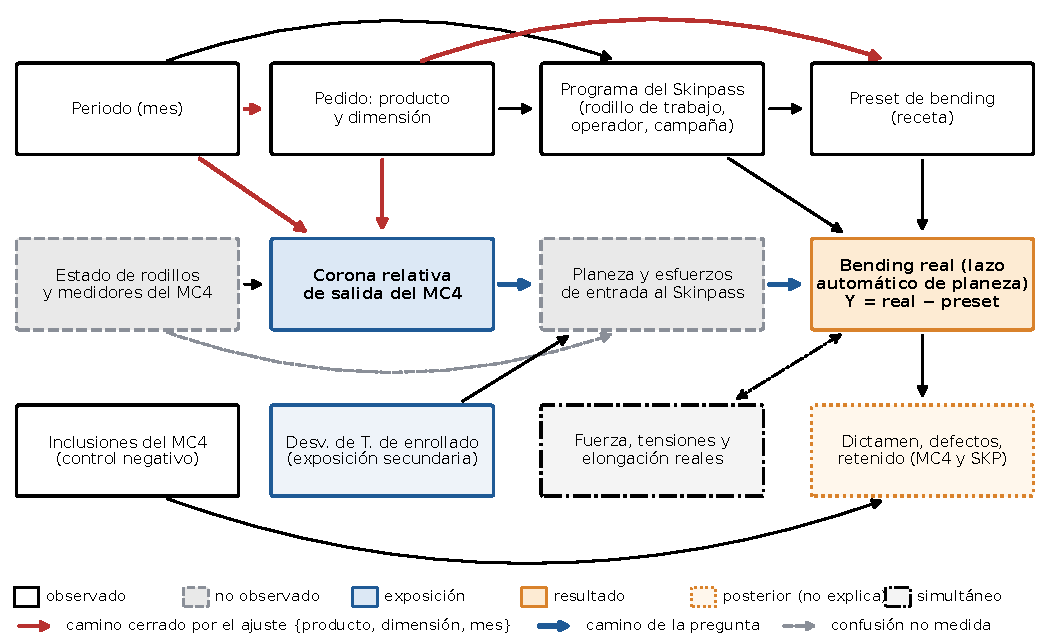
\includegraphics[width=\textwidth]{figuras/diagrama_causal.pdf}
\caption{\textbf{Ajustar por producto, dimensión y mes cierra los caminos de confusión observados entre la corona del
MC4 y la corrección de bending; la planeza de entrada y el estado de los rodillos quedan sin medir.} Pregunta que
responde: ¿qué hay que ajustar para comparar rollos con distinta corona, y qué no podemos ver? Cada flecha dice ``esto
influye en aquello''. Respecto a la Entrega~I se agregan el periodo, el programa del Skinpass, el preset dentro de un
lazo cerrado y la planeza de entrada, y se corrige el orden: el Skinpass va antes del decapado.}
\label{fig:dag}
\end{figure*}

La Fig.~\ref{fig:dag} resume lo que sabemos del proceso. El pedido (producto y dimensión) fija la corona que
el MC4 apunta a entregar y la receta del Skinpass; el periodo cambia la mezcla de pedidos, el estado del molino y de
sus medidores, y la programación. Esos dos caminos (en rojo) hacen que, sin ajuste, comparar rollos con distinta corona
sea comparar pedidos y meses distintos. El conjunto de ajuste que se desprende del diagrama es, por eso,
\{producto, dimensión, mes\}, que implementamos como efectos fijos de celda. El programa del Skinpass influye en el
preset y en el bending real pero no en la corona con que el rollo sale del MC4, de modo que no confunde la asociación
corona~$\rightarrow$~$\Y$: lo usamos para agrupar la incertidumbre y como fuente de variación en la descomposición, no
como ajuste. Quedan sin medir la planeza de entrada al Skinpass, el estado de los rodillos de ambos molinos y las
decisiones del operador; la sección~\ref{sec:validacion} acota cuánto podrían cambiar la conclusión. La
Tabla~\ref{tab:variables} resume el papel de cada variable.

\begin{table*}[t]
\centering
\caption{Variables y sus papeles en el diagrama causal. ``Ajuste'' indica si la variable entra al conjunto de ajuste
de la asociación corona~$\rightarrow$~$\Y$.}
\label{tab:variables}
\footnotesize
\begin{tabular}{L{3.6cm}L{4.1cm}L{1.6cm}L{6.9cm}}
\toprule
Variable & Papel en el diagrama & Ajuste & Por qué \\
\midrule
Producto, dimensión & Confusor (el pedido fija la corona y la receta) & Sí & Abre los caminos pedido $\rightarrow$ corona y pedido $\rightarrow$ preset \\
Mes & Confusor (mezcla de pedidos, estado de medidores) & Sí & La corona y la corrección cambian durante el año \\
Programa del Skinpass & Fuente de variación de $\Y$ & No (agrupa errores) & No causa la corona; se usa en la descomposición y para agrupar la incertidumbre \\
Corona relativa del MC4 & Exposición principal & --- & Corona / espesor, en puntos porcentuales; continua, sin cortes convencionales \\
Desv. de T. de enrollado & Exposición secundaria & --- & Real menos objetivo (°C) \\
Preset de bending & Componente de $\Y$ & No & Usarlo como explicativa crea un acoplamiento mecánico con $\Y$ \\
Fuerza, tensiones y elongación reales & Respuestas simultáneas & No & Se generan en el mismo proceso que $\Y$ \\
Dictamen, defectos, retención & Posteriores al resultado & No & Etiquetas derivadas, en buena parte por regla \\
Inclusiones del MC4 & Control negativo & No & Nacen en el acero, aguas arriba; no deberían responder al Skinpass \\
Acuñamiento (cuña) & Comprobación & Solo en R7 & Ternium indicó que no es prioritario \\
\bottomrule
\end{tabular}
\end{table*}

La exposición principal es la corona relativa, la corona de salida dividida entre el espesor y expresada en puntos
porcentuales (pp) del espesor (mediana \CoronaRelMediana\,\%), como variable continua, sin los cortes convencionales
de la Entrega~I. La cuña sale de la pregunta: Ternium indicó que no es prioritaria y en la exploración no se asoció
con la corrección de forma consistente; se conserva solo como comprobación. Seis supuestos sobre el significado de las
columnas, que ya no podemos confirmar con el Socio Formador, se escriben con su evidencia y su prueba de sensibilidad
en el Anexo~\ref{sec:anexo-supuestos}; los dos más importantes son que el preset está en kN como el bending real y que
un preset de cero significa ``sin preset'' (\PctPresetCero\,\% de los rollos).

\subsection{Análisis}
\label{sec:analisis}

\paragraph{Soporte} Antes de estimar, contamos por producto los rollos, programas, meses y celdas con al menos cinco
rollos, y la variación de la corona relativa dentro de celda. Un producto sin variación de corona dentro de celda no
aporta a la asociación y sale con nota.

\paragraph{Descomposición} Para cada nivel $\ell$ de la jerarquía tipo~$\rightarrow$~producto~$\rightarrow$~dimensión
$\rightarrow$~programa~$\rightarrow$~rollo calculamos la fracción de la suma de cuadrados de $\Y$ que explica,
\begin{equation}
f_\ell = \frac{\sum_i \left(\bar{\Y}_{c_\ell(i)} - \bar{\Y}_{c_{\ell-1}(i)}\right)^2}{\sum_i \left(\Y_i - \bar{\Y}\right)^2},
\label{eq:descomp}
\end{equation}
donde $c_\ell(i)$ es la celda del rollo $i$ en el nivel $\ell$. Con grupos pequeños cualquier agrupación parece explicar
mucho, así que cada fracción se compara con la que daría el azar, permutando 100 veces las etiquetas del nivel dentro de
su celda padre; reportamos el \emph{exceso sobre el azar}, $f_\ell$ menos la media nula. Su intervalo de 95\,\% se
obtiene de 200 réplicas en las que se toma al azar la mitad de los programas, sin reemplazo. Elegimos este método en
lugar del bootstrap con reemplazo porque duplicar programas sesga las fracciones de suma de cuadrados (bitácora del
plan). La descomposición se repite con el programa antes que el producto, para mostrar cuánto depende del orden, y
con el día, la semana y el rodillo de trabajo en lugar del programa.

\paragraph{Asociación} Estimamos
\begin{equation}
\Y_i = \beta\, \mathrm{corona}_i + \gamma\, \Delta T_i + \alpha_{c(i)} + \varepsilon_i ,
\label{eq:fe}
\end{equation}
con efectos fijos $\alpha_c$ de celda, la desviación de la temperatura de enrollado $\Delta T_i$ como exposición
secundaria y errores agrupados por programa del Skinpass, con corrección CR1 que cuenta los efectos fijos
absorbidos~\cite{cameron2015}. Reportamos $\beta$ en kN por punto porcentual de corona relativa y por una desviación
estándar de la corona dentro de celda, su $R^2$ parcial y la curva de $\Y$ por deciles de la corona, ambas centradas en
su celda. La misma especificación, con el preset como resultado, comprueba que la receta no reacciona a la corona del
rollo. Para la heterogeneidad estimamos la misma pendiente dentro de cada producto con al menos 300 rollos (efectos fijos
de dimensión por mes) y controlamos la tasa de descubrimientos falsos~\cite{benjamini1995}.

\paragraph{Predicción} Para saber si la información previa al Skinpass permite \emph{anticipar} $\Y$, comparamos un
solo modelo de aprendizaje automático, \emph{gradient boosting} con producto, dimensión, tipo, mes, corona relativa,
desviación de temperatura de enrollado y objetivos de espesor, ancho y temperatura, contra una línea base sencilla: la
media de $\Y$ por producto y dimensión en entrenamiento, que es lo que haría una receta por producto. Ambos se evalúan
con la misma validación: cinco particiones agrupadas por programa (ningún programa queda dividido) y una partición
temporal (entrenar con los programas de enero a agosto y evaluar de septiembre a noviembre)~\cite{roberts2017}. Una
validación aleatoria se reporta solo para mostrar cuánto infla el desempeño mezclar rollos de un mismo programa. Los
hiperparámetros se eligen dentro de cada partición de entrenamiento. Antes de correr el modelo fijamos qué cuenta como
mejora clara: bajar el error absoluto medio (MAE) en las cinco particiones agrupadas y en la temporal. La importancia de
cada variable, por permutación, describe lo que el modelo usa para predecir y no un efecto~\cite{shmueli2010}.

\subsection{Validación y sensibilidad}
\label{sec:validacion}
Sin verdad de terreno, sometimos la asociación a cuatro anclajes, cada uno con lo que la habría refutado, escrito antes
de verlo. \textbf{V1, control negativo}~\cite{lipsitch2010}: las inclusiones del MC4 nacen en el acero y no deberían
asociarse con $\Y$; habría refutado la conclusión una asociación con intervalo que excluya cero y magnitud comparable a
la de la corona. \textbf{V2, consistencia física}: una banda con más corona relativa necesita un claro entre rodillos
más abierto al centro, y el doblado positivo de los rodillos de trabajo cierra el centro, de modo que el lazo debería
responder con un bending más negativo; este argumento mecánico es nuestro (la literatura revisada no fija el signo), y
lo habría refutado una pendiente positiva con intervalo que excluya cero. \textbf{V3, robustez}~\cite{steegen2016}:
nueve decisiones de depuración razonables (R1~umbral de corona imposible; R2~definición de producto; R3~corte de
censura; R4~rollos divididos; R5~preset cero; R6~rollos sin el Skinpass en la ruta; R7~cuña como covariable; R8~presets
mayores que el máximo bending real; R9~rodillo de trabajo en lugar de programa), mostradas juntas; la habría refutado un
cambio de signo de la pendiente o que el producto superara al programa. \textbf{V4, programa contra periodo}: sustituir
el programa por el día o la semana; no refuta, pero si da lo mismo hay que escribir ``programa o periodo''. Para la
confusión no medida reportamos el valor de robustez de Cinelli y Hazlett~\cite{cinelli2020}, la proporción de la
varianza residual de la exposición y del resultado que un confusor tendría que explicar para anular la pendiente, y lo
comparamos con el del producto como confusor observado de referencia. Todos los contrastes examinados (\NContrastes)
están en la tabla completa del repositorio (Anexo~\ref{sec:anexo-contrastes}).

\section{Resultados}
\label{sec:resultados}

\subsection{Soporte}
\label{sec:res-soporte}

\begin{table*}[tb]
\centering
\caption{\textbf{Hay variación de la corona dentro de celda en los tres tipos de material, y todos los productos con
300 rollos o más tienen soporte para la asociación.} Celdas: producto $\times$ dimensión $\times$ mes. DE corona:
desviación estándar de la corona relativa dentro de celda, en puntos porcentuales del espesor, ponderada por rollos
(celdas con dos o más rollos). Prod.\ $\geq$300: productos con al menos 300 rollos.}
\label{tab:soporte}
\footnotesize
\begin{tabular}{lrrrrrrrr}
\toprule
Tipo & Rollos & Progr. & Prod. & Prod. $\geq$300 & Celdas & \% en celdas $\geq$5 & DE corona (pp) & \% preset 0 \\
\midrule
CALIENTE & 16,456 & 746 & 152 & 12 & 2,070 & 84.6 & 0.69 & 11.6 \\
DECAPADO & 27,177 & 754 & 234 & 23 & 4,457 & 79.6 & 0.53 & 11.1 \\
FRIO & 639 & 121 & 31 & 0 & 136 & 77.2 & 0.38 & 0.0 \\
Total & 44,272 & 831 & 331 & 35 & 6,137 & 83.2 & 0.60 & 11.1 \\
\bottomrule
\end{tabular}

\end{table*}

La Tabla~\ref{tab:soporte} resume el diagnóstico de soporte, hecho antes de cualquier estimación. Los
\NProdGrandes{} productos con al menos 300 rollos reúnen el \PctRollosProdGrandes\,\% de la población y todos tienen
variación de corona dentro de celda; los \NSinSoporte{} productos sin esa variación suman solo \NSinSoporteRollos{}
rollos y salen de la asociación. La corona relativa varía \SDCoronaDentro{}~pp (una desviación estándar) dentro de su
celda, y \PctPresetCero\,\% de los rollos tiene un preset de cero. El análisis de la asociación usa
\NAsocRollos{} rollos en \NAsocCeldas{} celdas con al menos dos rollos y \NAsocProgramas{} programas.

\subsection{De dónde viene la corrección de bending}
\label{sec:res-descomp}

\begin{figure*}[tb]
\centering
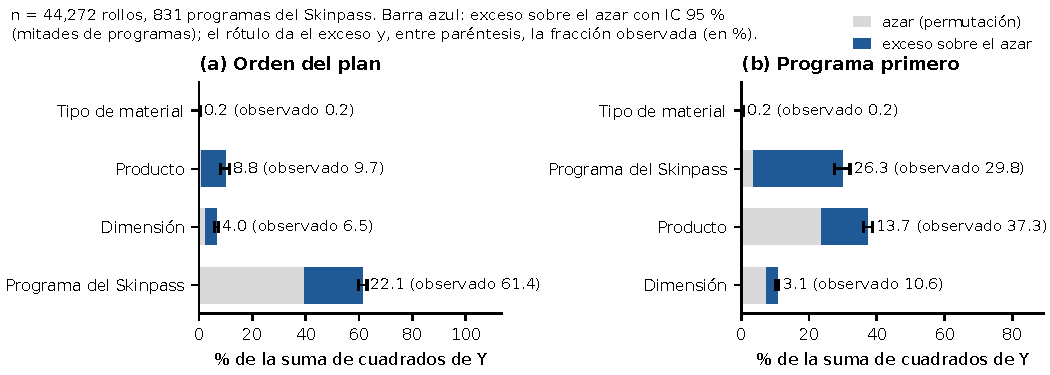
\includegraphics[width=\textwidth]{figuras/fig_r1_descomposicion.pdf}
\caption{\textbf{La corrección de bending varía más entre programas del Skinpass que entre productos, en cualquier
orden de la descomposición.} Pregunta que responde: ¿qué parte de las diferencias de $\Y$ entre rollos se explica por
el tipo de material, el producto, la dimensión y el programa, más allá de lo que daría el azar? Cada barra es la
fracción de la suma de cuadrados de $\Y$ que explica un nivel (ec.~\ref{eq:descomp}); la parte gris es la que el mismo
nivel obtendría con etiquetas permutadas, así que solo cuenta el tramo azul. (a) Orden del plan. (b) Programa antes que
producto.}
\label{fig:descomp}
\end{figure*}

La corrección de bending tiene mediana de \YMediana~kN (percentiles 5 y 95: \YPcinco{} y \YPnoventaycinco~kN): en la
mayoría de los rollos el bending real queda por debajo del preset de la receta. La Fig.~\ref{fig:descomp}
reparte su variación. En el orden del plan, el programa del Skinpass explica \ObsPrograma\,\% de la suma de cuadrados,
pero el azar ya explicaría \NulaPrograma\,\% por el tamaño pequeño de sus grupos dentro de cada producto y dimensión:
su exceso sobre el azar es de \ExcesoPrograma~puntos (IC~95\,\% \ExcesoProgramaIC). El producto aporta
\ExcesoProducto~puntos \ExcesoProductoIC, la dimensión \ExcesoDimension{} \ExcesoDimensionIC{} y el tipo de material
\ExcesoTipo. Producto y dimensión juntos suman \ExcesoProdDim~puntos, menos que el programa solo. Con el programa antes
que el producto (Fig.~\ref{fig:descomp}b), el programa aporta \ExcesoAltPrograma~puntos y el producto \ExcesoAltProducto:
el orden cambia las cifras, pero no cuál pesa más.

\subsection{Corona del MC4 y corrección de bending}
\label{sec:res-corona}

\begin{figure*}[tb]
\centering
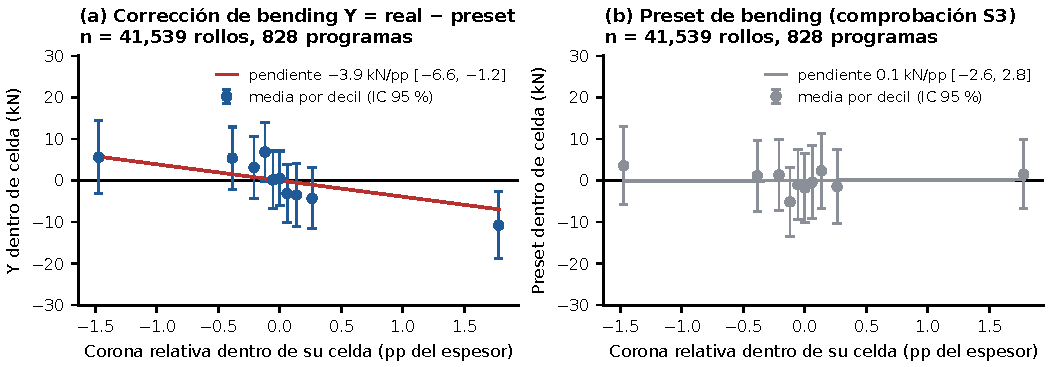
\includegraphics[width=\textwidth]{figuras/fig_r2_corona.pdf}
\caption{\textbf{Más corona relativa de salida del MC4 se asocia con una corrección de bending más negativa, con una
magnitud pequeña; el preset no responde a la corona.} Pregunta que responde: dentro de un mismo producto, dimensión y
mes, ¿los rollos que salen del MC4 con más corona reciben una corrección distinta? Ambos ejes están centrados en la
celda del rollo. Cada punto es la media de un decil de corona, con su IC~95\,\% agrupado por programa; la recta es la
pendiente de la ec.~\ref{eq:fe}. (a) Corrección $\Y$. (b) Preset, como comprobación de que la receta no reacciona a la
corona del rollo.}
\label{fig:corona}
\end{figure*}

Dentro de celda, cada punto porcentual adicional de corona relativa se asocia con una corrección de bending
\PendCorona~kN más negativa (IC~95\,\% \PendCoronaIC; $t=\PendCoronaT$ con errores agrupados por programa), es decir,
\PendCoronaSD~kN por una desviación estándar de corona dentro de celda \PendCoronaSDIC. La corona explica
\RParcialCorona\,\% de la varianza de $\Y$ que queda dentro de celda ($R^2$ parcial). La curva por deciles
(Fig.~\ref{fig:corona}a) es aproximadamente lineal, sin un umbral, y las diferencias entre deciles son de pocos kN.
La desviación de la temperatura de enrollado no se asocia con $\Y$ (\PendTemp~kN por °C, \PendTempIC). El preset no
responde a la corona del rollo (\PendPreset~kN por punto, \PendPresetIC; Fig.~\ref{fig:corona}b).

Con la misma especificación, el bending real se mueve igual que la corrección (\SecBendReal~kN por punto), lo que
descarta que la asociación dependa de las unidades del preset. Los indicadores secundarios no se mueven con la corona:
por cada punto porcentual, el porcentaje de rollos con defecto de inspector cambia \SecDefInsp~puntos porcentuales,
el de rollos retenidos \SecRetenido{} y la elongación lograda \SecElong~puntos de elongación.

\subsection{Heterogeneidad entre productos}
\label{sec:res-het}

\begin{figure}[t]
\centering
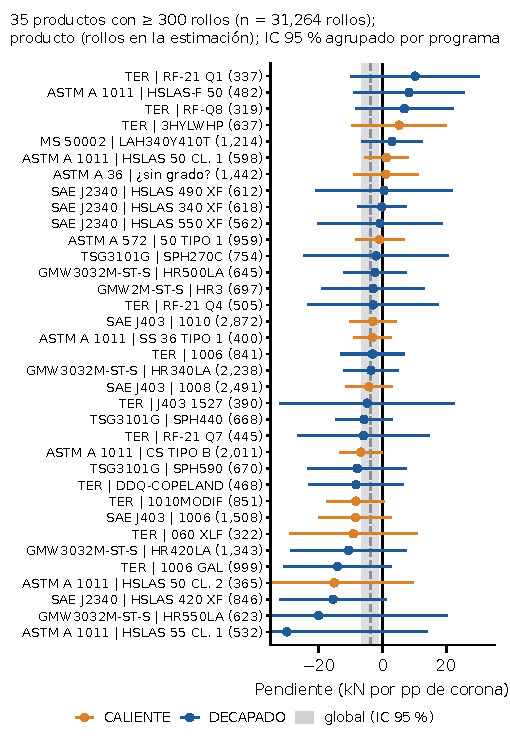
\includegraphics[width=\columnwidth]{figuras/fig_r3_productos.pdf}
\caption{\textbf{Ningún producto muestra una pendiente corona~$\rightarrow$~$\Y$ distinta de cero después de controlar
la tasa de descubrimientos falsos.} Pregunta que responde: ¿la asociación es igual en todos los productos? Cada
renglón es un producto con al menos 300 rollos (entre paréntesis, rollos en la estimación), con su pendiente e
IC~95\,\% agrupado por programa. Están todos, no solo los extremos; la franja gris es la estimación global.}
\label{fig:productos}
\end{figure}

La Fig.~\ref{fig:productos} muestra la pendiente en cada uno de los \NProdHet{} productos con al menos 300 rollos
(\NProdHetRollos{} rollos). \NProdNeg{} de las \NProdHet{} pendientes son negativas, como la global; van de
\PendProdMin{} a \PendProdMax~kN por punto, con intervalos anchos. Solo \NProdICexcluyeCero{} intervalo excluye el cero
y, al controlar la tasa de descubrimientos falsos al 5\,\%, \NProdBH{} productos se distinguen de cero.

\subsection{Validación y sensibilidad}
\label{sec:res-validacion}

\begin{figure*}[tb]
\centering
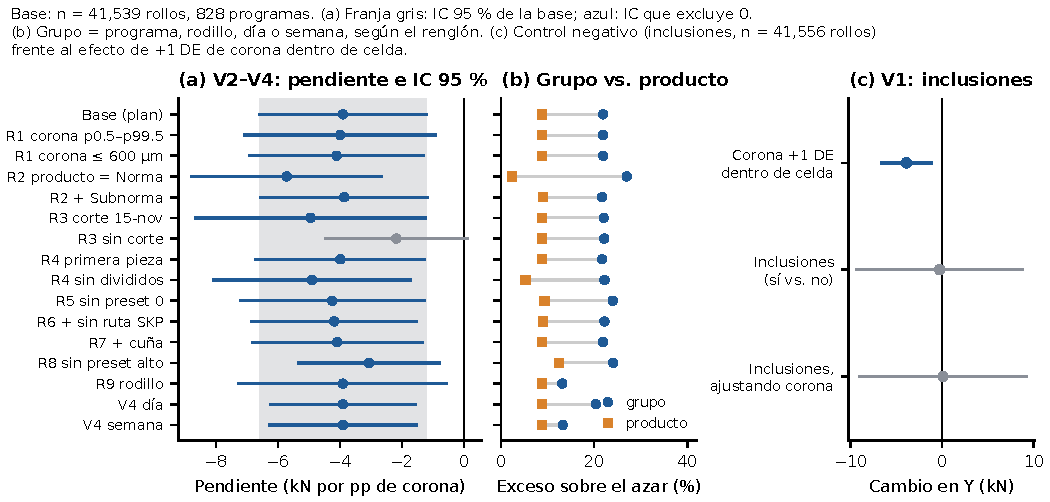
\includegraphics[width=\textwidth]{figuras/fig_r4_validacion.pdf}
\caption{\textbf{La dirección de la asociación y el predominio del programa sobre el producto sobreviven a
\NVariantes{} alternativas, y el control negativo no responde.} Pregunta que responde: ¿la conclusión depende de una
decisión de depuración, de la forma de agrupar o de una confusión que un control negativo detectaría? (a) Pendiente de
corona con su IC~95\,\% en cada alternativa (una sola decisión cambia por renglón; V4 agrupa la incertidumbre por día o
semana). (b) Exceso sobre el azar del grupo (programa, rodillo, día o semana) y del producto en la descomposición. (c)
Asociación de las inclusiones del MC4 con $\Y$, junto al efecto de una desviación estándar de corona.}
\label{fig:validacion}
\end{figure*}

\paragraph{V1, control negativo} Las inclusiones del MC4 (\NInclusiones{} rollos, \PctInclusiones\,\%) no se asocian
con la corrección: \VUnoCoef~kN \VUnoIC{} sin ajustar por la corona y \VUnoCoefAj~kN \VUnoICAj{} ajustando por ella
(Fig.~\ref{fig:validacion}c). El intervalo es amplio porque las inclusiones son raras; no excluye un efecto del tamaño
del de la corona, pero tampoco lo sugiere.

\paragraph{V2, consistencia física} El signo es el esperado (más corona, bending más negativo) y su intervalo excluye el
cero. La magnitud es pequeña: pasar del percentil 10 al 90 de la corona dentro de celda (de \VDosPdiez{} a
\VDosPnoventa~pp) cambia la corrección en \VDosCambio~kN, frente a una desviación estándar de \YDEAsoc~kN y un rango
intercuartil del bending real de \BendRealIQR~kN.

\paragraph{V3, robustez} Ninguna de las \NVariantes{} alternativas cambia el signo de la pendiente, que va de
\PendMvMin{} a \PendMvMax~kN por punto (Fig.~\ref{fig:validacion}a). Un intervalo, el de la alternativa sin corte de
censura, incluye el cero (\NVariantesICCero{} de \NVariantes): al incluir diciembre la pendiente se acerca a cero. En
todas las alternativas el grupo (programa, rodillo, día o semana) explica más que el producto
(Fig.~\ref{fig:validacion}b): el exceso del producto va de \ExcProdMvMin{} a \ExcProdMvMax~puntos y el del grupo de
\ExcGrupoMvMin{} a \ExcGrupoMvMax.

\paragraph{V4, programa contra periodo} Agrupar por día del Skinpass en lugar de por programa da casi lo mismo
(\VCuatroExcesoDia~puntos \VCuatroExcesoDiaIC, contra \VCuatroExcesoProg~\VCuatroExcesoProgIC{} del programa). Por
semana (\VCuatroExcesoSemana) y por rodillo de trabajo (\VCuatroExcesoRodillo) el exceso baja, pero sigue por encima
del producto (\VCuatroProductoProg).

\paragraph{Confusión no medida} El valor de robustez de la pendiente es de \CHRV\,\%: un confusor no medido que explique
esa proporción de la varianza residual de la corona y de la corrección bastaría para anularla (\CHRVa\,\% para que su
intervalo incluya el cero). El producto, el confusor observado de referencia, explica \CHRDRef\,\% de la varianza de la
corona y \CHRYRef\,\% de la de la corrección (dentro de dimensión y mes). Un confusor con solo \CHKAnula{} veces la fuerza
del producto, aproximadamente 1/\CHUnoEntre, bastaría para anular la pendiente.

\subsection{Predicción}
\label{sec:res-prediccion}

\begin{figure}[t]
\centering
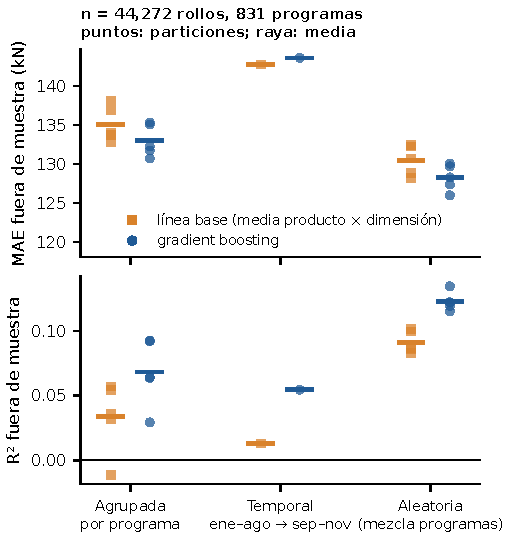
\includegraphics[width=\columnwidth]{figuras/fig_r5_prediccion.pdf}
\caption{\textbf{Con validación agrupada y temporal, el modelo no anticipa la corrección claramente mejor que una
receta por producto y dimensión.} Pregunta que responde: ¿la información disponible antes del Skinpass permite
anticipar $\Y$? Error absoluto medio (arriba) y $R^2$ fuera de muestra (abajo) de la línea base (media por producto
$\times$ dimensión) y del modelo, en cada partición. La validación aleatoria mezcla rollos de un mismo programa y se
muestra solo para ver cuánto infla el desempeño.}
\label{fig:prediccion}
\end{figure}

En las cinco particiones agrupadas por programa, el modelo baja el error absoluto medio de \PredMAEBaseGrupo{} a
\PredMAEModGrupo~kN (diferencia de \PredMAEDifGrupo~kN, DE \PredMAEDifGrupoDE{} entre particiones; mejora en
\PredMejoraGrupo{} de 5). En la partición temporal, entrenado con \PredNTempTrain{} rollos de enero a agosto y evaluado
en \PredNTempTest{} de septiembre a noviembre, el modelo es peor que la línea base en error absoluto medio
(\PredMAEModTemp{} contra \PredMAEBaseTemp~kN), aunque su $R^2$ es mayor (\PredRModTemp{} contra \PredRBaseTemp).
Por el criterio fijado antes de correrlo, no hay mejora clara. Ambos explican poco: el $R^2$ fuera de muestra del modelo
es de \PredRModGrupo{} en la validación agrupada (Fig.~\ref{fig:prediccion}). La validación aleatoria, que mezcla
rollos de un mismo programa, sube el $R^2$ de los dos (\PredRBaseAleat{} y \PredRModAleat). Lo que el modelo usa para
predecir es sobre todo el producto: permutarlo sube el error en \PredImpPrimeraKN~kN, contra \PredImpCorona~kN de la
corona, la segunda variable.

Por último, para dimensionar la propuesta de validación, estimamos con las mismas particiones agrupadas cuánto bajaría
el trabajo del lazo, $|\Y|$, si el preset se recentrara con la mediana histórica de la corrección. Con la receta
vigente, $|\Y|$ promedia \ExpAbsY~kN fuera de muestra; recentrar el preset por producto y dimensión lo bajaría
\ExpDeltaA~kN (DE \ExpDeltaADE{} entre particiones), y recentrarlo con una sola mediana global, \ExpDeltaGlobal~kN.
Diferenciar por producto agregaría \ExpDeltaDif~kN (DE \ExpDeltaDifDE) a recentrar la receta única.

\section{Discusión}
\label{sec:discusion}

Organizamos la discusión en cuatro hallazgos. Para cada uno decimos qué encontramos, qué implica para la decisión de
Ternium, qué no implica y qué dato o experimento cerraría la brecha. Los cuatro viven en los dos primeros peldaños de
la escalera de afirmaciones: \emph{observamos} y \emph{se asocia, ajustando por}.

\subsection{H1. La corrección depende más del programa, o del periodo, que del producto}
\emph{Qué encontramos.} Por encima del azar, el programa del Skinpass explica \ExcesoPrograma~puntos de la variación de
la corrección de bending \ExcesoProgramaIC, el producto \ExcesoProducto{} \ExcesoProductoIC{} y la dimensión
\ExcesoDimension; el predominio del programa se mantiene si entra antes que el producto y en las \NVariantes{}
alternativas de depuración y agrupación y agrupación. Agrupar por día da casi lo mismo que por programa (\VCuatroExcesoDia{} puntos).

\emph{Qué implica.} Una receta por producto podría absorber, como máximo, la parte sistemática de la corrección que
viaja con el producto: \ExcesoProducto{} puntos de su suma de cuadrados por encima del azar (\ExcesoProdDim{} con la
dimensión). La parte más grande cambia de un programa a otro o de un día a otro, y ninguna receta por producto la
absorbería. Para decidir, lo que más pesa es qué cambia entre programas: el rodillo de trabajo, el operador, la mezcla
de pedidos del periodo o el estado de los medidores.

\emph{Qué no implica.} No implica que el programa cause la corrección: con estos datos, el programa y el día son casi
indistinguibles, por lo que escribimos ``programa o periodo''. Tampoco implica que los productos respondan distinto a la
receta. Que un producto necesite en promedio una corrección distinta es una diferencia de \emph{nivel}; que necesite
una receta distinta exige una diferencia de \emph{respuesta}, es decir, que el mismo cambio de receta tenga efectos
distintos en productos distintos, y eso no se observa en datos donde la receta casi no varía dentro de producto. Por
último, no implica que reducir la corrección mejore la calidad: el Skinpass no registra planeza de salida.

\emph{Qué lo cerraría.} El registro, por rollo, de la campaña de rodillos de trabajo (hoy solo el identificador del
rodillo), de los cambios de receta con su fecha de vigencia y de los ajustes manuales del operador con su motivo
permitiría separar el programa del periodo. El experimento de la sección~\ref{sec:experimento} bloquea ese efecto en
lugar de estimarlo.

\subsection{H2. La corona del MC4 se asocia con la corrección, pero poco y de forma frágil}
\emph{Qué encontramos.} Dentro de producto, dimensión y mes, un punto porcentual más de corona relativa se asocia con
una corrección \PendCorona~kN más negativa \PendCoronaIC, con el signo que predice el argumento mecánico. El control
negativo no responde, la dirección sobrevive a \NVariantes{} alternativas y el preset no reacciona a la corona. Pero el
efecto es pequeño: del percentil 10 al 90 de la corona la corrección cambia \VDosCambio~kN, frente a una desviación
estándar de \YDEAsoc~kN. Además es frágil: un confusor no medido con 1/\CHUnoEntre{} de la fuerza del producto bastaría
para anularlo.

\emph{Qué implica.} La forma con que el rollo sale del MC4 lleva poca información útil para fijar el preset del
Skinpass. Ajustar el preset por la corona movería la corrección unos pocos kN, una fracción pequeña del trabajo que
hoy hace el lazo (\ExpAbsY~kN de $|\Y|$ promedio).

\emph{Qué no implica.} No es un efecto causal, y la fragilidad lo impide aún más que de costumbre: la planeza de
entrada y el estado de los rodillos del MC4 influyen tanto en la corona como en lo que el lazo necesita corregir. Tampoco
implica que la corona no importe para la planeza final: el lazo compensa la forma de entrada, y lo que medimos es cuánto
la compensó, no si la compensación fue suficiente.

\emph{Qué lo cerraría.} Una medición de planeza a la entrada del Skinpass, que hoy no existe, convertiría a la principal
variable no medida del diagrama en una variable observada.

\subsection{H3. No se detectan diferencias de respuesta entre productos}
\emph{Qué encontramos.} De los \NProdHet{} productos con al menos 300 rollos, \NProdNeg{} tienen una pendiente
corona~$\rightarrow$~$\Y$ negativa como la global, pero ninguno se distingue de cero tras controlar la tasa de
descubrimientos falsos y los intervalos se traslapan ampliamente.

\emph{Qué implica.} Con estos datos no hay evidencia de que algún producto reaccione a la forma de entrada de manera
distinta a los demás. Es la única forma de interacción que podemos estimar, y no aparece.

\emph{Qué no implica.} No demuestra que los productos respondan igual: con intervalos de este ancho, la ausencia de
evidencia no es evidencia de equivalencia, que exigiría fijar un margen de equivalencia de antemano~\cite{wellek2010}.
Los productos de los extremos de la Fig.~\ref{fig:productos} son los peores candidatos para una receta especial: con
\NProdHet{} comparaciones, el más extremo sobrestima su efecto por la maldición del optimizador~\cite{smith2006}.

\emph{Qué lo cerraría.} Variación deliberada del preset dentro de producto, que solo puede venir de un experimento.

\subsection{H4. La información previa al Skinpass no anticipa la corrección mejor que una receta por producto}
\emph{Qué encontramos.} El modelo de gradient boosting baja el error absoluto medio \PredMAEDifGrupo~kN respecto a la
media por producto y dimensión en la validación agrupada, pero es peor en la temporal, y los dos explican menos del
10\,\% de la variación fuera de muestra. Lo que el modelo usa es, sobre todo, el producto. Recentrar el preset con la
mediana histórica bajaría $|\Y|$ unos \ExpDeltaA~kN; casi todo eso (\ExpDeltaGlobal~kN) se logra con una sola mediana
global, y diferenciar por producto agregaría \ExpDeltaDif~kN.

\emph{Qué implica.} Optimizar el preset con un modelo más flexible sobre la información previa al Skinpass agregaría muy
poco a una receta por producto, y una receta por producto agregaría muy poco a recentrar la receta única. Lo que sí
sugieren los datos es que la receta vigente está desplazada (la corrección mediana es de \YMediana~kN), y esa es una
hipótesis operativa que vale la pena probar.

\emph{Qué no implica.} No implica que la corrección sea impredecible con otros datos; el modelo no conoce la planeza de
entrada ni el estado de los rodillos. Tampoco implica que un preset recentrado mejore la calidad: el lazo corrige de
todos modos, y la ganancia, si la hay, estaría en el tramo de cabeza del rollo, antes de que el lazo converja. Los datos
resumidos por rollo no separan ese tramo.

\emph{Qué lo cerraría.} El experimento de la sección~\ref{sec:experimento}, con planeza de salida medida durante su
ejecución.

\subsection{Relación con la literatura}
Los resultados coinciden con la advertencia de Box~\cite{box1966}: las variables latentes del proceso, aquí resumidas
en el programa o el periodo, pesan más que las variables observadas que solemos poner en un modelo, y la asociación de
la corona sería la conclusión equivocada de un análisis que no la sometiera a sensibilidad. También coinciden con la
física del temple~\cite{lenard2014} en que la forma de entrada importa (el signo de la asociación es el esperado),
pero matizan su alcance práctico: en una planta con un lazo de planeza, esa forma deja una huella pequeña en la
corrección. Y chocan con la expectativa, común en la literatura de aprendizaje automático en manufactura~\cite{wuest2016},
de que un modelo más flexible extraerá de los datos de proceso lo que una regla simple no ve: con validación por
programa y por tiempo, la ventaja casi desaparece, como advierten Roberts et al.~\cite{roberts2017}.

\subsection{Limitaciones, escritas como hallazgos}
\begin{itemize}
\item \emph{Sin resultado de forma.} El Skinpass no registra planeza. Sus defectos de inspector afectan al
      \PctDefInspector\,\% de los rollos y el \PctTensionEnrollado\,\% de esos registros son de tensión de enrollado, no
      de forma; por eso no pudimos usar la calidad de forma como resultado.
\item \emph{Censura de fin de año.} Solo \PctDicEnSKP\,\% de los rollos de diciembre llega al Skinpass de 2025, y los de
      diciembre traen más corona (\CoronaRelMedianaDic\,\% contra \CoronaRelMediana\,\%). Sin el corte, la pendiente se
      acerca a cero y su intervalo lo incluye.
\item \emph{La receta no es tan única.} El preset es único en el \PctPresetUnicoTodos\,\% de los grupos programa
      $\times$ producto $\times$ dimensión, pero solo en el \PctPresetUnicoDos\,\% de los que tienen dos o más rollos;
      \PctPresetCero\,\% de los rollos tiene preset cero y \NPresetAlto{} rollos tienen un preset mayor que el máximo
      bending real observado. Las unidades del preset son un supuesto (Anexo~\ref{sec:anexo-supuestos}).
\item \emph{Programa y periodo, indistinguibles.} El día explica \VCuatroExcesoDia{} puntos contra
      \VCuatroExcesoProg{} del programa.
\item \emph{Confusión fuerte por pedido.} El producto explica \CHRDRef\,\% de la varianza de la corona dentro de
      dimensión y mes; cualquier confusor parecido, aunque mucho más débil, cambiaría la conclusión sobre la corona.
\item \emph{Un año, una planta, un resumen por rollo.} No sabemos qué resume cada valor (promedio, punta u otro) ni
      separamos el enhebrado del tramo estable.
\end{itemize}

\section{Conclusiones y propuesta de validación}
\label{sec:conclusiones}

En un año de rollos ligados entre el MC4 y el Skinpass de Pesquería, la corrección que el lazo de bending aplica sobre
la receta depende más del programa del Skinpass, o del periodo en que se procesa el rollo, que del producto: el
programa explica \ExcesoPrograma~puntos de su variación por encima del azar y el producto \ExcesoProducto. La corona con
que el rollo sale del MC4 se asocia con la corrección en la dirección física esperada, pero con una magnitud pequeña y
frágil, y la información previa al Skinpass no la anticipa claramente mejor que una receta por producto. Antes de
diferenciar recetas por producto, por lo tanto, proponemos validar con un experimento dentro de cada programa y
registrar la planeza de salida.

\paragraph{Contribución} Para Ternium, el artículo acota lo que una receta por producto podría absorber de la
corrección del Skinpass y muestra que la mayor parte de esa corrección cambia de un programa o de un día a otro; además
deja una unión verificada entre ambos molinos, reproducible con un solo comando. Para el campo, muestra cómo plantear
una pregunta respondible cuando la pregunta original exige un resultado que la planta no mide, y cómo someter una
asociación de planta a control negativo, multiverso y sensibilidad antes de traducirla en una decisión.

\subsection{Experimento propuesto}
\label{sec:experimento}
Proponemos una operación evolutiva~\cite{box1957}: perturbaciones pequeñas, dentro del rango ya operado, que no
detienen la producción.
\begin{itemize}
\item \emph{Qué se asigna.} Factor A: preset vigente frente a preset recentrado con la mediana histórica de la
      corrección de su celda producto $\times$ dimensión, limitado al rango de preset ya usado en esa celda. Factor B,
      sin costo adicional en un diseño factorial $2^2$: ajuste del preset por la corona relativa del MC4.
\item \emph{Unidad y bloqueo.} El rollo, alternado dentro de cada programa del Skinpass en bloques permutados de cuatro
      y estratificado por celda~\cite{box2005,montgomery2017}. Asignar por rollo y no por programa es la consecuencia
      práctica de H1: bloquear por programa elimina de la comparación la fuente de variación más grande. Es viable porque
      el preset ya cambia entre rollos de un mismo programa.
\item \emph{Resultado y criterio de decisión, fijados antes.} Resultado primario: $|\Y|$ promedio, en kN. Se adopta el
      recentrado si baja $|\Y|$ al menos \ExpDeltaA~kN con un intervalo que excluya cero y si ningún indicador
      secundario empeora más que un margen de no inferioridad acordado con Ternium~\cite{wellek2010}. Indicadores
      secundarios: defectos de inspector, rollos retenidos, elongación lograda, la cola (porcentaje de rollos con $|\Y|$
      mayor que su percentil 90 histórico) y, si se instala, la planeza de salida.
\item \emph{Volumen.} Con una desviación estándar de $|\Y|$ dentro de programa y celda de \ExpTodoSigmaDentro~kN, detectar
      \ExpDeltaA~kN con 80\,\% de potencia y $\alpha=0.05$ requiere \ExpTodoARollos{} rollos, unas \ExpTodoASemRollo{}
      semanas de producción del Skinpass (\ExpTodoRollosSemana{} rollos por semana). Asignar por programa requeriría
      \ExpTodoAProg{} programas (unas \ExpTodoASemProg{} semanas). Limitado a la familia más grande
      (\ExpFamilia, \ExpFamiliaRollos{} rollos al año), tomaría unas \ExpFamASemRollo{} semanas. Con ese volumen, el
      factor B solo se detectaría si su efecto fuera de al menos \ExpMDEB~kN, el doble del estimado.
\item \emph{Lo que el volumen revela.} Para probar lo que diferenciar por producto agrega al recentrado de la receta
      única (\ExpDeltaDif~kN) harían falta \ExpTodoDifRollos{} rollos, más de una década de producción. Ese es un
      hallazgo en sí mismo: con lo que hoy se mide, la diferenciación por producto no se puede validar
      experimentalmente en un plazo razonable, y no es donde está la mayor parte de la corrección.
\item \emph{Reglas de paro.} Revisión semanal por el ingeniero de proceso del Skinpass, que decide. Se detiene un
      brazo si su tasa de defectos de inspector supera a la del otro en más de un punto porcentual dos semanas seguidas, o
      si aparece un defecto de forma (fuera de planeza, ondulación, tableado) en rollos consecutivos del mismo brazo.
\end{itemize}

\subsection{Datos del Skinpass que harían respondible la pregunta original}
\begin{enumerate}
\item \emph{Planeza de salida} como medición continua a lo ancho, por rollo, con el tramo estable separado del enhebrado
      y la aceleración. Sin ella no hay un resultado de forma que comparar entre recetas.
\item \emph{Forma de entrada}, aunque sea una medición gruesa: es el principal confusor no medido del diagrama.
\item \emph{Consigna y valor medido de cada palanca} (bending, elongación, fuerza, tensiones, velocidad) a lo largo del
      rollo, y la \emph{lógica de los lazos}: qué actuador responde a qué medición. Sin esto no se distinguen las
      palancas de los mediadores.
\item \emph{Campaña de rodillos de trabajo} de cada rollo (fecha de montaje y toneladas acumuladas), el \emph{historial
      de recetas} con fechas de vigencia y los \emph{ajustes del operador} con su motivo.
\item \emph{El mismo identificador} que usa el MC4: con él ligamos el \PctCalienteEnSKP--\PctDecapadoEnSKP\,\% de los
      rollos planeados para el Skinpass. Las señales de 2026 que recibimos durante la Entrega~I no coincidían con ningún
      rollo de 2025, así que cualquier dato nuevo debe cubrir el mismo periodo que el registro del MC4.
\end{enumerate}
Una advertencia acompaña esta lista: mientras exista una receta por tipo de material, la variación de configuración
dentro de cada producto será pequeña y en buena parte reactiva. Los registros históricos, aun completos, medirán bien
cuánto difieren los productos en lo que llegan necesitando, pero la diferencia de respuesta, que es lo que justificaría
una receta por producto, casi con seguridad exigirá un experimento diseñado en el Skinpass.

En suma, es verdad que la corrección del Skinpass depende más del programa o del periodo que del producto, y poco de la
forma con que el rollo sale del MC4. Sigue sin saberse si reducir esa corrección mejora la planeza y si algún producto
responde distinto a la receta. Lo resolvería un experimento rollo a rollo dentro de cada programa, con la planeza de
salida medida.


\section*{Disponibilidad de datos y código}
Los datos pertenecen a Ternium y están bajo acuerdo de confidencialidad. El código, el plan de análisis con su
bitácora, las tablas agregadas y la tabla completa de \NContrastes{} contrastes examinados están en el repositorio
del equipo; un solo comando (\texttt{python -m src.reproducir}) regenera todas las figuras, tablas y cifras de este
artículo a partir de los 36 archivos originales.

\bibliographystyle{elsarticle-num}
\bibliography{referencias}

\onecolumn
\appendix
\section{Diccionario razonado de las variables que usa el análisis}
\label{sec:anexo-diccionario}
La Tabla~\ref{tab:diccionario} lista las variables que entran al análisis. El diccionario completo del MC4 (76
variables) está en el repositorio (\texttt{outputs/tablas/diccionario\_razonado.csv}). \emph{Estado}: observado
(verificado en los datos), inferido (interpretación nuestra) o supuesto (sin confirmación posible; Anexo~\ref{sec:anexo-supuestos}).

\begin{table}[!h]
\centering
\caption{Diccionario razonado. Fuente: MC4 (archivos MC4\_PSQ) o SKP (archivos SKP\_PSQ). Tipo: especificación (se fija
antes de producir), medición, etiqueta (la calcula el sistema o la asigna un inspector) o identificador.}
\label{tab:diccionario}
\footnotesize
\begin{tabular}{L{3.2cm}cL{4.4cm}cL{1.8cm}L{2.5cm}c}
\toprule
Variable (columna) & Fuente & Qué es & Unidad & Tipo & Papel & Estado \\
\midrule
Material Salida / Material Entrada & MC4 / SKP & Identificador del rollo; llave de la unión & --- & identificador & llave & observado \\
Programa & SKP & Tanda de rollos procesados de corrido en el Skinpass (mediana \MedianaRollosPrograma) & --- & identificador & grupo, agrupación de errores & inferido \\
Rodillo de Trabajo & SKP & Rodillo de trabajo montado (\NRodillos{} rodillos) & --- & identificador & alternativa al programa (R9) & observado \\
Norma, Grado & MC4 & Estándar del acero y su variante; juntos son el producto & --- & especificación & confusor & observado \\
Espesor y Ancho Objetivo & MC4 & Dimensión pedida, en rangos & mm & especificación & confusor & observado \\
Fecha Inicio & MC4 & Inicio de laminación; da el mes y el corte de censura & --- & medición & confusor (periodo) & observado \\
Corona Salida, Espesor & MC4 & Corona de salida y espesor medido; su cociente es la corona relativa & µm, mm & medición & exposición & supuesto (S6) \\
Temp Enrollado Real y Obj & MC4 & Temperatura de enrollado real y objetivo & °C & medición / esp. & exposición secundaria & observado \\
Defecto (i) = INCLUSIONES & MC4 & Defecto con origen en el acero & --- & etiqueta & control negativo & observado \\
Acuñamiento Salida & MC4 & Cuña de salida & µm & medición & comprobación (R7) & supuesto \\
Preset Bending & SKP & Bending fijado por la receta & kN & especificación & componente de $\Y$ & supuesto (S1, S2) \\
Bending Prom. Real [kN] & SKP & Bending real promedio aplicado por el lazo & kN & medición & componente de $\Y$ & observado \\
Fuerza, Tensiones reales & SKP & Fuerza de laminación y tensiones promedio & kN & medición & simultáneas (no entran) & observado \\
Elongación, Modo Molino & SKP & Elongación lograda; modo fuerza o elongación & \%, --- & medición & indicador secundario & observado \\
Registro Automatico (i), Linea Origen (i) & SKP & Si el defecto lo puso el sistema y en qué línea nació & --- & etiqueta & define el indicador de inspector & observado \\
Dictamen & SKP & ACEPTADO, RETENIDO o REPROCESO & --- & etiqueta & indicador secundario & observado \\
Peso & SKP & Peso de cada pieza; pondera la agregación por rollo & kg & medición & ponderador & observado \\
\bottomrule
\end{tabular}
\end{table}

\section{Preguntas al Socio Formador y supuestos}
\label{sec:anexo-supuestos}
En la Entrega~I, Ternium respondió dos preguntas: el acuñamiento de un solo lado no es una prioridad operativa (por
eso salió de la pregunta) y compartió señales de bending del Skinpass de 2026 a 25~Hz, que no coinciden con ningún
rollo de 2025 y quedaron fuera de alcance. Las demás preguntas (qué resume cada valor, unidades, registro de rodillos,
reglas automáticas) ya no pueden consultarse; cada una se convirtió en un supuesto explícito con su evidencia y su
prueba de sensibilidad (Tabla~\ref{tab:supuestos}).

\begin{table}[!h]
\centering
\caption{Supuestos, evidencia en los datos y prueba de sensibilidad.}
\label{tab:supuestos}
\footnotesize
\begin{tabular}{cL{3.5cm}L{6.6cm}L{2.9cm}L{2.6cm}}
\toprule
& Supuesto & Evidencia & Si es falso & Sensibilidad \\
\midrule
S1 & El preset está en kN, como el bending real & Misma escala (percentiles 1--99: preset \PresetPuno{} a \PresetPnoventaynueve; real \RealPuno{} a \RealPnoventaynueve~kN); el real sigue al preset (pendiente \PendRealPreset, $r=\CorrRealPreset$) & $\Y$ mezclaría unidades & R8; el bending real (sin preset) da la misma pendiente \\
S2 & Preset cero significa ``sin preset'' & \PctPresetCero\,\% de los rollos; con preset cero el bending real sigue activo (mediana \BendRealPresetCero~kN; exactamente cero en \PctRealCeroPresetCero\,\%) & $\Y$ sería otra cosa en esos rollos & R5 \\
S3 & El preset se fija antes del rollo y no reacciona a él & Único en \PctPresetUnicoTodos\,\% de los grupos programa $\times$ producto $\times$ dimensión (\PctPresetUnicoDos\,\% con dos o más rollos); no responde a la corona (\PendPreset~kN/pp) & El preset sería una respuesta & Se describe; afecta la lectura \\
S4 & El programa agrupa rollos con el mismo rodillo de trabajo & \PctProgUnRodillo\,\% de los programas usa un solo rodillo; mediana de \MedianaProgRodillo{} programas por rodillo & El programa no reflejaría el rodillo & R9 \\
S5 & El bending real responde a un lazo de planeza & El real se aparta del preset (mediana de $\Y$: \YMediana~kN; $|\Y|>50$~kN en \PctYMayorCincuenta\,\%) & El bending sería una decisión manual & Se describe en el diagrama \\
S6 & La corona está en µm & Mediana \CoronaMedianaUm~µm (p5--p95: \CoronaPcincoUm--\CoronaPnoventaycincoUm) con espesor mediano de \EspesorMediano~mm: corona relativa de \CoronaRelMediana\,\% & Cambia la escala de la pendiente, no su signo & Pendiente también por DE \\
\bottomrule
\end{tabular}
\end{table}

\section{Tabla completa de contrastes examinados}
\label{sec:anexo-contrastes}
Examinamos \NContrastes{} contrastes. Cada uno, con su estimación, intervalo, unidades, valor $p$, valor $q$ de
Benjamini--Hochberg cuando corresponde, rollos y grupos, está en \texttt{outputs/tablas/contrastes\_completos.csv}. La
Tabla~\ref{tab:contrastes} los resume por familia; en el cuerpo del artículo solo aparecen los que contestan la pregunta.

\begin{table}[!h]
\centering
\caption{Resumen de los contrastes por familia. Mín.\ y Máx.: rango de las estimaciones en la familia. IC excluye 0:
cuántos intervalos de 95\,\% excluyen el cero. $q_{\min}$: menor valor $q$ de Benjamini--Hochberg.}
\label{tab:contrastes}
\footnotesize
\begin{tabular}{L{4.6cm}rrrlrL{4.2cm}}
\toprule
Familia & $n$ & Mín. & Máx. & IC excluye 0 & $q_{\min}$ & Unidades \\
\midrule
8.B descomposición (orden del plan) & 4 & 0.22 & 22.07 & 3 de 4 & -- & \% de la SC de Y \\
8.B descomposición (programa primero) & 4 & 0.22 & 26.29 & 3 de 4 & -- & \% de la SC de Y \\
V4 programa vs. periodo & 4 & 13.23 & 22.07 & 4 de 4 & -- & \% de la SC de Y \\
8.C asociación principal & 2 & −3.90 & −0.23 & 1 de 2 & -- & kN por unidad \\
Indicadores secundarios & 10 & −3.78 & 0.12 & 2 de 10 & -- & por unidad de la exposición \\
8.D heterogeneidad por producto & 35 & −30.04 & 10.24 & 1 de 35 & 0.70 & kN por pp \\
V1 control negativo & 2 & −0.27 & 0.09 & 0 de 2 & -- & kN \\
V3 robustez: pendiente de corona & 16 & −5.71 & −2.18 & 15 de 16 & -- & kN por pp \\
V3 robustez: exceso del grupo − producto & 16 & 4.34 & 24.73 & -- & -- & puntos de \% de la SC \\
10 confusión no medida & 1 & 1.47 & 1.47 & -- & -- & \% de varianza residual \\
8.E predictivo & 6 & −2.21 & 0.84 & -- & -- & kN (media entre particiones) \\
12 experimento: tamaño del efecto & 4 & 0.82 & 8.04 & -- & -- & kN (media de 5 particiones agrupadas) \\
\bottomrule
\end{tabular}

\end{table}

\section{Plan de análisis}
\label{sec:anexo-plan}
El plan (\texttt{docs/plan\_de\_analisis.md}) fijó, antes de la estimación principal, la pregunta y la afirmación más fuerte
que esperábamos sostener, la unión y la población con sus exclusiones, el resultado y los indicadores secundarios, el
conjunto de ajuste derivado del diagrama, el diagnóstico de soporte, los análisis, los cuatro anclajes de validación
con sus criterios de refutación, las nueve alternativas de robustez y los seis supuestos. Su bitácora registra, con fecha
y motivo, los cambios posteriores. Los principales: el intervalo del exceso sobre el azar se calcula con mitades de
programas en lugar de bootstrap con reemplazo (el bootstrap se conserva en el repositorio); se definió de antemano qué
cuenta como mejora clara del modelo predictivo; el signo físico esperado se presenta como argumento mecánico del equipo,
porque la referencia prevista no lo confirma; y la propuesta de experimento, escrita después de ver los resultados,
agrega el factor de recentrado por producto y cambia la unidad de asignación del programa al rollo dentro de programa.


\end{document}
